\documentclass[]{report}
\usepackage{graphicx, float,}
\usepackage{hyperref}
\usepackage[export]{adjustbox}

\title{\centering CSP334 : Computer Networks \\Lab Assignment No 6\\Assignment on DNS}
\author{\LARGE Sahil\\2016UCS0008}

% to use proper section numbering in the report type 
\renewcommand{\thesection}{\arabic{section}}

\begin{document} 

\maketitle

%%%%%%%%%%%%%%%%%%%%%%%%%%%%%%%%%%%%%%%%%%%%%%%%
\section{SET 1: The Basic DNS:}

\subsection{:}
\large
The transport layer protocol used for sending the DNS queries is \textbf{UDP}.
\\
\textbf{Benefits of UDP:} There is no connection establishment in UDP, so there is no need to maintain connection state. Hence, it is a simple protocol. 
\\
Also, data is not retransmitted if there is any loss of data, which can be used in time sensitive applications like real-time audio or video. 
\\
\textbf{Drawbacks of UDP:} Data loss can occur as it does not provide reliability. Also, no timing and minimum throghput guarantees are provided.

\subsection{:}
\begin{figure}[H]
	\vspace{0pt}
	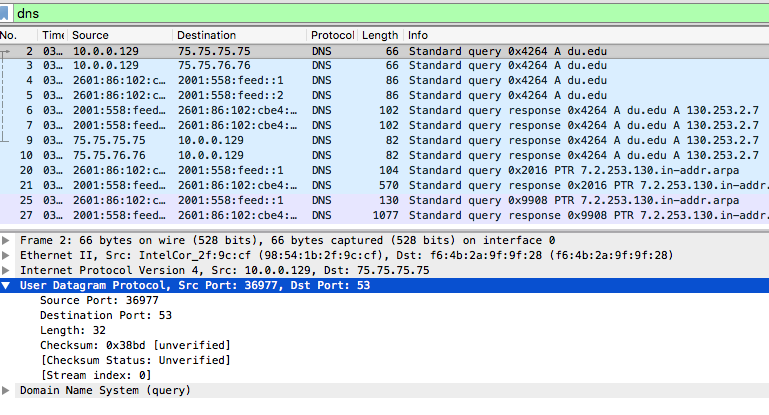
\includegraphics[height = 250pt, keepaspectratio]{Snapshots/1_2.png}
\end{figure}

The port numbers used for sending the packet is $36977$ and receiving the packet is $53$. 

\subsection{:}
- The destination of packet $2$ is $75.75.75.75$. \\
- It is a DNS query of type \textbf{A} as shown. In this, we give the hostname in the query and receive the IPA in the response. 
\\
\begin{figure}[H]
	\vspace{0pt}
	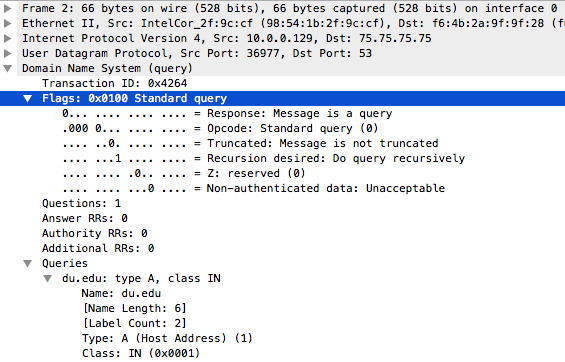
\includegraphics[height = 200pt, keepaspectratio]{Snapshots/1_3_1.png}
\end{figure}
- The only flag set in the query is \textbf{recursion desired}.
\\
- To know the type of DNS server, we check the response to this query. 
\begin{figure}[H]
	\vspace{0pt}
	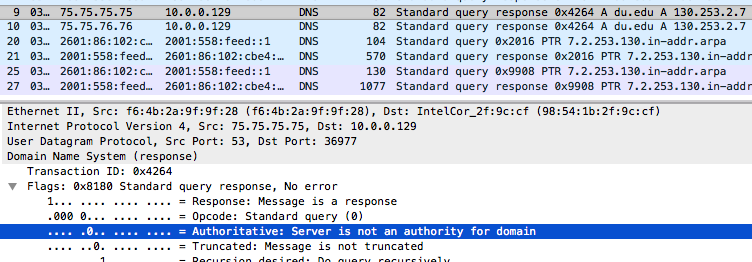
\includegraphics[height = 150pt, keepaspectratio]{Snapshots/1_3_2.png}
\end{figure}
In the response, the flag \textbf{authoritative} is not set. Thus, it must be a local server having the IPA of the hostname cached. 

\subsection{:}



\section{SET 2: Using the DNS\_2.pcapng:}

%%%%%%%%%%%%%%%%%%%%%%%%%%%%%%%%%%%%%%%%%%%%%%%%

\end{document}